% !TEX root = ..\thesis.tex

\chapter{TỔNG QUAN}
\section{Giới thiệu vấn đề}
\subsection{Vấn đề phân loại rác thải sinh hoạt}
% Phân loại rác cụ thể là làm gì? Các "class" hay các "loại" rác cần phải phân loại là gì, có ý nghĩa gì với môn trường, với cuộc sống
Phân loại rác bao gồm nhận diện, mô tả các loại chất thải dựa trên nguồn gốc và đặc điểm và phân loại chúng vào những danh mục rác khác nhau và theo những phương pháp phân loại khác nhau, có thể diễn ra theo phương thức thủ công tại nhà hoặc được thu gom bởi dịch vụ hoặc được phân loại tự động bằng máy. Mỗi danh mục rác đã phân loại sẽ được xử lý bằng những cách khác nhau, miễn là có lợi cho môi trường và cho cuộc sống người dân. Việc phân loại đóng vai trò thiết yếu trong một hệ thống quản lý và thu gom rác thải, đơn giản và thuận tiện hóa quá trình xử lý rác của các cơ sở thu gom rác, nâng cáo ý thức người dân và giúp nhà nước quản lý những rủi ro thiệt hại tới sức khỏe con người và môi trường sống.

Nhìn chung, rác thải sẽ được phân loại làm 3 loại chính, được thể hiện như bảng \ref{tab.garbage.type}

\begin{table}[H]
    \centering
    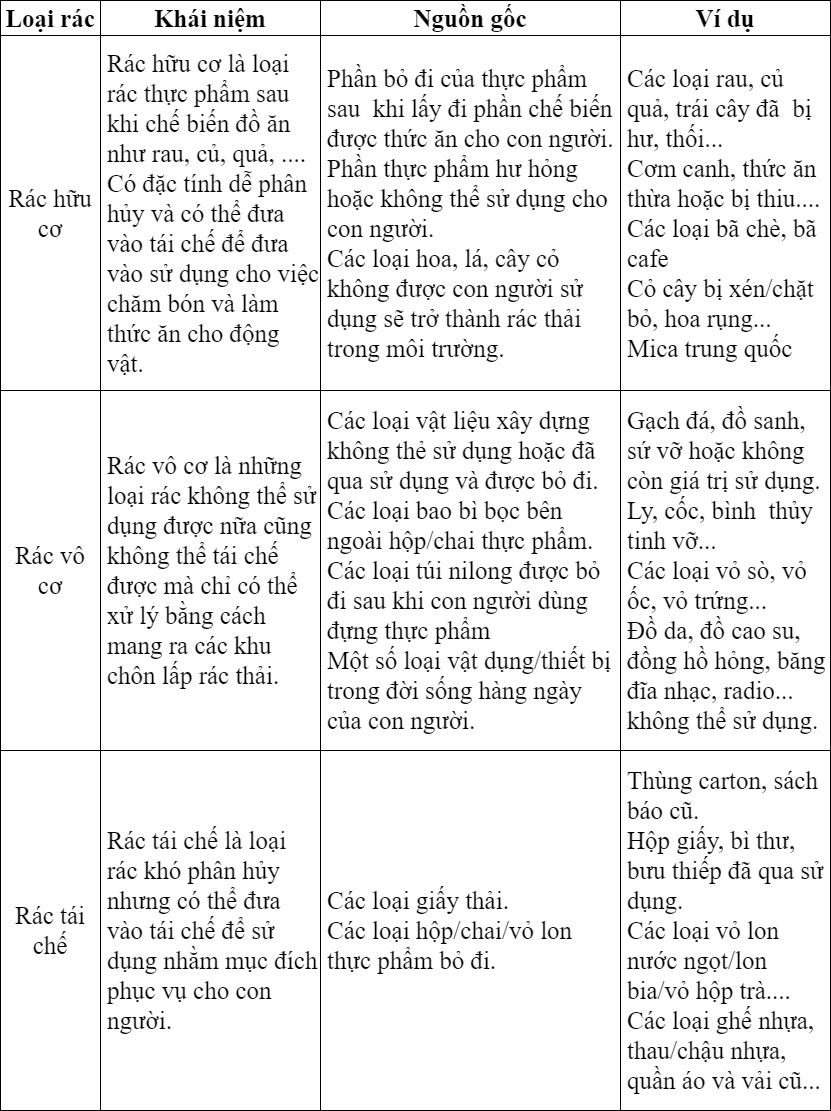
\includegraphics[width=\textwidth]{images/TraditionalTrash.png}
    \caption{Các loại rác truyền thống} 
    \label{tab.garbage.type}
\end{table}
Trong 3 loại chính, người ta còn định nghĩa cụ thể những loại rác khác:

% sửa cụ thể các loại rác thải thuộc loại nào.
\begin{itemize}
    \item Rác thải văn phòng: những văn phòng phẩm không còn được sử dụng (giấy báo cũ,  bút hết mực, …)
    \item Rác thải công nghiệp: loại rác có thành phần cực kỳ độc thải ra từ các nhà máy, công xưởng,… (chất ngâm tẩm, tẩy rửa, chất hóa học, phế liệu công nghiệp, thuốc trừ sâu bọ, thuốc kích thích tăng trưởng…) 
    \item Rác thải xây dựng: loại rác được thải ra môi trường từ những công trình xây dựng, sửa chữa, còn được gọi là xà bần (gạch, đá, vụn đất, …)
    \item Rác thải y tế: loại rác được thải ra từ các cơ sở y tế, bệnh viện, bệnh xá, được phân loại cụ thể như sau:
   \begin{itemize}
    \item Chất thải y tế lây nhiễm: gồm các chất thải lây nhiễm sắc nhọn (kim tiêm, lưỡi dao mỗ, đinh, cưa, kim chọc dò, …) và không sắc nhọn (chất thải thấm, dính máu hoặc dịch sinh học cơ thể, chất thải phát sinh từ buồng cách ly, …), chất thải có nguy cơ lây nhiễm cao (mẫu bệnh phẩm, dụng cụ đựng, dính mẫu bệnh phẩm phát sinh từ các phòng xét nghiệm an toàn sinh học …) và chất thải giải phẫu (mô, bộ phận cơ thể người thái bỏ và xác động vật thí nghiệm)
    \item Chất thải y tế nguy hại không lây nhiễm: gồm hóa chất, dược phẩm thải bỏ có các thành phân nguy hại, thiết bị y tế vỡ, hỏng, đã qua sử dụng có chứa thủy ngân hoặc kim loại nặng, chất hàn răng amalgam thải bỏ
    \item Chất thải y tế thông thường: gồm chất thải rắn trong sinh hoạt thường ngày của con người, chất thải ngoại cảnh trong cơ sở y tế và chất thải lỏng không nguy hại.
   \end{itemize}   
\end{itemize}

Vì thế, việc phân loại rác mang một vài ý nghĩa quan trọng đối với môi trường tự nhiên và cộng đồng xã hội:
\begin{itemize}
    \item Nhằm giảm thiểu tổng lượng rác thải từ cộng đồng ra môi trường do đó góp phần làm không khi trong lành và giảm thiểu nguy cơ ô nhiễm môi trường. 
    \item Giảm thiểu nguy cơ phát tán các tác nhân gây bệnh, các yếu tố độc hại, nguy hiểm. 
    \item Hạn chế nước rỉ rác góp phần làm giảm ô nhiễm nguồn đất, nguồn nước ngầm, nước mặt, giảm nhiều diện tích chôn lắp rác sinh hoạt. 
    \item Ngoài ra, phân loại rác còn có ảnh hưởng đến chất lượng cuộc sống của con người đem lại một lượng lớn các sản phẩm tái chế, mang lại hiệu quả kinh tế cho chính người thải rác bằng cách bán các nguyên, phế liệu có thể tái chế được, tận dụng các nguyên liệu hữu cơ sản xuất phân bón vi sinh.
    \item Góp phần nâng cao ý thức cuộc của cộng đồng về bảo vệ môi trường cũng như sử dụng tài nguyên hợp lý, nhất là ở trẻ nhỏ.
    \item Xây dựng một xã hội với môi trường xanh-sạch-đẹp.
    \item Nhằm giảm tải công tác xử lý, nhất là trong phương pháp đốt chất thải, đồng thời có thể lựa chọn phương pháp xử lý chất thải rắn phù hợp nhất.
    \item Giảm thiểu tổng lượng rác thải ra môi trường tiết kiệm chi phí thu gom, vận chuyển và xử lý.    
\end{itemize}

% Các cách phân loại rác truyền thống hiện nay là gì? (nói thêm về quy trình xử lí rác thải, từ việc thu gôm đến cách xử lí của nhà máy, chôn đốt rác plapaa => gây ảnh hưởng đến môi trường.)

Trước đây, quá trình phân loại rác thải sẽ do các cơ sở thu gom rác thực hiện nhưng vì tổng lượng rác thải từ nhiều nguồn được thải ra ngày càng nhiều nên việc huy động người dân phân loại rác tại nguồn là cách được sử dụng rộng rải nhất. Cách phân loại sẽ tùy thuộc vào mỗi địa phương quy định chi tiết, ở Việt Nam sẽ chia thành 3 danh mục: rác vô cơ, rác hữu cơ và rác tái chế. Các cơ sở thu gom rác sẽ tiến hành thu gom tận nơi và vận chuyển đến điểm tập trung, lượng rác được phân loại sẽ được xử lý theo 3 phương pháp sau:
\begin{itemize}
    \item Chế biến rác thải thành phân compost: chế biến rác hữu cơ dễ phân hủy thành phân compost dùng trong nông nghiệp, chia thành 2 quy mô chế biến:
        \begin{itemize}
            \item Quy mô chế biến tập trung: Rác hữu cơ dễ phân hủy được tách ly, nghiền, ủ hiếu khí để tạo ra phân vi sinh. Việc thành lập nhà máy chế biến phân compost cần vốn đầu tư lớn, chi phí vận hành cũng tương đối cao.
            \item  Quy mô chế biến hộ gia đình: Rác hữu cơ dễ phân hủy được ủ thành phân compost ngay trong sân vườn
        \end{itemize}

    \item Chôn lấp hợp vệ sinh: Rác thải được rải thành từng lớp dưới hố, đầm nén để giảm thể tích và phủ đất lên (phun  hóa chất để tăng hiệu quả xử lý nhanh và hạn chế côn trùng) với sơ đồ quy định như hình \ref{fig:so_do_chon_lap}:
    
        \begin{figure}[H]
            \centering            
            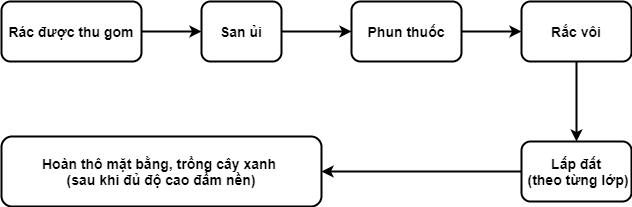
\includegraphics[width=\textwidth]{images/SoDoChonLap.png}
            \caption{Sơ đồ chôn lấp \cite{trashclassification}}
            \label{fig:so_do_chon_lap}
        \end{figure}

    \item Thiêu đốt: Rác thải được phân hủy ở nhiệt độ cao (1000 – 1100°C), giảm đáng kể thể tích chất thải phải chôn lấp (xỉ, tro), tuy nhiên chi phí đầu tư, vận hành nhà máy đốt rác khá cao, phù hợp với các nước tiên tiến, phát triển. 
   

\end{itemize}
Ngoài ra, một số khu vực khác sẽ có cách phân loại rác theo 4 loại lớn: 
    \begin{itemize}
        \item Rác dễ cháy (rác thải từ nhà bếp, giấy vụn, vải quần áo).
        \item Rác khó cháy (kim loại, thủy tinh, sành sứ).
        \item Rác tái chế (chai, bình, can, giấy báo).
        \item Rác cỡ lớn (đồ gia dụng cỡ lớn).
    \end{itemize}
  

Đồng nghĩa với việc rác thải được phân chia vào từng loại khác nhau, là tính chất của các loại rác cũng sẽ khác nhau. Như vậy, từng loại phải có cách xử lý riêng.

Mỗi địa phương sẽ quy định chi tiết cách phân loại rác khác nhau, nhưng cách truyền thống nhất nhất và được sử dụng rộng rãi nhất là chia rác thành 3 danh mục: rác vô cơ, rác hữu cơ và rác tái chế.
Ngoài ra, một số khu vực khác sẽ có cách phân loại rác theo 4 loại lớn: rác dễ cháy (rác thải từ nhà bếp, giấy vụn, vải quần áo), rác khó cháy (kim loại, thủy tinh, sành sứ), rác tái chế (chai, bình, can, giấy báo) và rác cỡ lớn (đồ gia dụng cỡ lớn)

\subsection{Phân loại sử dụng Internet of Things}
% Internet of things là gì 
Internet of Things (IoT) là một hệ sinh thái (được gọi là \qq{thiết bị kết nối} và \qq{thiết bị thông minh}), nhà cửa và các trang thiết bị khác được nhúng với các bộ phận điện tử, phần mềm, cảm biến, cơ cấu chấp hành cùng với khả năng kết nối mạng máy tính giúp cho các thiết bị này có thể thu thập và truyền tải dữ liệu
% Sự phổ biến của IoT 
Internet of Things đang dần trở nên quen thuộc và trở thành một trong số các trào lưu của nền công nghiệp hóa 4.0.
Không khó để có thể bắt gặp những sản phẩm thuộc lĩnh vực này, từ những sản phẩm gần gũi trong đời sống gia đình như đèn điều khiển bằng âm thanh, cửa thông minh...cho đến các sản phẩm giúp ích trong nông nghiệp như hệ thống tưới tiêu cho hoa màu từ xa, theo dõi các yếu tố về môi trường .... 
% Ưu điểm phân loại rác kết hợp IoT
Chưa dừng lại ở đó, khi xã hội càng phát triển, việc kết hợp các phần kiến thức độc lập với nhau thành một thể thống nhất để nâng cao chất lượng của sản phẩm tạo ra là điều hết sức cần thiết.
Điều đó được chứng minh rõ ràng qua việc bắt đầu có các sản phẩm IoT sử dụng kỹ thuật Machine Learning được ra đời và ứng dụng vào các lĩnh vực, vấn đề mà xã hội đang quan tâm.
Trong đó, bằng cách tạo ra các sản phẩm sử dụng công nghệ tiên tiến nói trên vào mục đích bảo vệ môi trường đang là một trong các ý tưởng thiết thực, đáp ứng nhu cầu của xã hội.
 
%Sửa so sánh với cái chung 
Ở các nước khác, việc cung cấp các loại thùng rác với từng loại rác đã trở nên phổ biến, và yêu cầu mọi người phải tự giác thực hiện việc bỏ rác đúng quy định, đúng thùng rác. Một số ví dụ cụ thể như:
Ở Nhật, việc bỏ rác được quy định ngay trên các tấm lịch, người dân cần phân loại rác và bỏ rác đúng loại rác vào ngày được quy định trên lịch nếu trường hợp ở hộ gia đình. Và các thùng rác công cộng cũng được kí hiệu phân loại rác, người dân phải bỏ đúng loại rác vào thùng rác có kí hiệu phân loại. Hoặc ở một số nước khác, như Singapore đã áp dụng các quy định cứng rắn đối với người dân và cả khách du lịch nếu họ vứt rác bừa bãi, mức phạt có thể lên đến 1,000 SGD (17 triệu đồng). Tuy nhiên, ở Việt Nam lại khá khó áp dụng như thế, về khách quan mà nói thì ta dễ dàng nhận thấy hệ thống thùng rác công cộng được bố trí trên đường khá thưa thớt, nên người dân khó tìm được nơi bỏ rác khi tham gia giao thông, và một mặt hạn chế mà chúng ta cần nhìn nhận là có một bộ phận không nhỏ người dân có ý thức chưa tốt, chưa thực hiện bỏ rác đúng nơi quy định cũng như chưa hình thành thói quen phân loại rác. Đa số  chúng ta đều để chung tất cả các loại rác thải vào một bao sau đó để nhân viên dọn vệ sinh gôm về nhà máy xử lý. Quy trình và các ảnh hưởng xấu của việc xử lí rác thải truyền thống như đã nêu ở mục trên, vì thế việc thiết kế thùng rác kết hợp IoT tự động phân loại rác và hệ thống quản lý vị trí thùng rác cũng như lượng rác trong mỗi thùng được cập nhật liên tục mỗi giờ sẽ mang lại rất nhiều lợi ích: Giảm bớt quy trình xử lý, giảm công sức lao động, giảm tiền của, và mang tính quản lý chủ động cao.



\section{Previous work}
% Đã có những đề tài, bài báo nào liên quan đến việc dùng IoT trong phân loại rác, tóm tắt nội dung từng bài. 4-5 bài là xong mục này,

% so sánh các ưu nhược điểm của các đề tài, họ làm được tới đâu.  
Trong công bố  \cite{trashnet}, hai tác giả đã cho rằng:

Dùng thị giác máy tính để phân loại tái chế rác sẽ mang lại nhiều hiệu quả đối với việc xử lý rác thải. Đối tưọng của bài toán này là dùng hình ảnh của một loại rác tái chế hoặc rác thải thông thường và phân loại chúng vào 6 lớp: thủy tinh, giấy, kim loại, nhựa, bìa cứng, và rác thải khác. Mindy Yang và Gary Thung cũng tạo ra một dataset bao gồm mỗi lớp khoảng 400 - 500 hình ảnh được thu thập một cách thủ công. Họ dự kiến công khai tập dataset cho cộng đồng. Hai model được sử dụng là: SVM (Support Vector Machine) với SIFT (Scale-Invariant Feature Transform) và CNN (Convolutional Neural Network). Các thử nghiệm của họ chỉ ra rằng SVM có hiệu quả cao hơn CNN. Tuy nhiên, CNN chưa được huấn luyện một cách tốt nhất do gặp nhiều khó khăn trong việc xác định siêu tham số.

Trong công bố  \cite{smartcity}, hai tác giả đã cho rằng:

Hiện nay, những khu đô thị, thành phố lớn đang dần được chuyển hóa để trở nên \qq{thông minh} hơn. Bên cạnh một số hệ thống quản lý thông minh phổ biến (giao thông, đèn, năng lượng, ...) thì hệ thống xử lý rác thải thông minh là một phần không thể thiếu cho bất kỳ một thành phố thông minh nào. 
Một hệ thống rác thải thông minh nhắm vào việc giải quyết lượng rác trong những khu công cộng hoặc ngoại ô. Ngoài việc mất mỹ quan đô thị của một khu vực, rác thải có thể gây ô nhiễm và ảnh hưởng trầm trọng đến chất lượng cuộc sống của người dân trong khu vực đó. Luận văn tập trung vào việc phát triển phần mềm có thể nhận diện lượng rác thải thông qua việc phân tích các luồng video ở thời gian thật. Mô hình mạng cải tiến YOLOv3 được triển khai để thực hiện chức năng phát hiện rác. Hệ thống đã được điều chỉnh thích hợp theo dataset đã được sưu tầm cho mục đích này.  

Kết quả cho thấy cách tiếp cận như trên đã đóng góp một phần to lớn vào việc quản lý rác thải hiệu quả hơn ở những thành phố thông minh.

Trong công bố \cite{lstmprediction1}, tác giả cho rằng dự báo chuỗi thời gian là một vấn đề quan trọng trong nhiều lĩnh vực, một dự đoán tốt chính là bằng chứng cốt yếu để mọi người đưa ra quyết định.

Đối với những mô hình thực hiện phương pháp dựa trên kiến thức thông kê, chúng hoạt động rất tốt với việc dự đoán một bước tiếp theo, nhưng khi tiến hành dự đoán nhiều bước tiếp, hiệu suất của một vài mô hình không đạt được như mong đợi. Vì thế, tác giả đã gợi ý sử dụng mô hình mạng LSTM (Long-Short Term Memory) để giải quyết bài toán mà không cần bận tâm đến nhiều bước thủ công trong các phương pháp mô hình hóa truyền thống, chẳng hạn như kiểm tra độ ổn định, hàm tự tương quan, hàm tự tương quan từng phần,...

Khi xét về chuỗi thời gian, có rất nhiều dữ liệu trong cuộc sống hằng ngày của chúng ta có thể được mô hình hóa thành chuỗi thời gian, như chỗ đậu xe còn lại trong bải đậu xe thay đổi theo giờ, số lượng khách đến bảo tàng mỗi ngày, chi phí điện cho trung tâm mua sắm hằng tháng,... Các chuỗi thời gian khác nhau có các đặc điểm khác nhau, một số có thể có giá trị trung bình xung quanh 0, một số có tính chất tuần hoàn, một số có tính chất tăng/giảm, cho nên xây dựng một mô hình phù hợp với nhiều loại chuỗi dữ liệu khác nhau là một nhiệm vụ khó khăn.

Kết quả bài báo cho thấy mô hình LSTM khá phù hợp với phạm vi rộng lớn các mẫu dữ liệu, nhưng các mẫu dữ liệu trong bài báo tương đối đơn giản và vẫn còn rất nhiều không gian khai thác trong lĩnh vực dữ đoán chuỗi thời gian đi trước nhiều bước.

\section{Mục tiêu nghiên cứu}
% Trên cơ sở vấn đề đã đặt, khóa luận dự kiến làm gì
%  Xây dựng thùng rác thông minh phân loại rác dựa trên hình. Mô tả kết cấu thùng, phân mấy loại rác, v.v...
%  Các chức năng xử về dữ liệu1
Nắm bắt xu thế trên, bài toán được đặt ra là phải tạo ra sản phẩm vừa đáp ứng được yêu dễ triển khai trên diện rộng, nhằm giảm sức người, tiết kiệm, mà người quản lý dễ kiểm soát, dễ sử dụng, sửa chữa.
Từ đó, đề tài về \qq{Xây dựng mô hình thùng rác thông minh dựa trên công nghệ trí tuệ nhân tạo} đã được ra đời để giải quyết bài toán đó. 
Thùng rác tự động phân loại rác áp dụng kỹ thuật Machine Learning để giảm thiểu thời gian, sức người cũng như các dây chuyển xử lí phân loại rác như trước đây, từ đó tiết kiệm được các khoản chi phí.
Tuy nhiên, việc thực hiện hóa đề tài trên đã gặp không ít nhũng khó khăn, để giảm thiểu chi phí thiết kế, cũng như hướng đến việc khả thi khi đưa vào thực tế.

Nhóm đưa ra phương hướng thiết kế phải đảm bảo các tiêu chí: giá thành hợp lí, tiết kiệm điện năng, và có thể sử dụng ở nhiều môi trường (đặc biệt là các khu vực khó cung cấp nguồn điện).
Để thực hiện các phương hướng đã đưa ra, nhóm chọn sử dụng mạch ESP32 CAM với giá thành cạnh tranh hơn rất nhiều so với sản phẩm dùng raspberry pi.
Ngoài ra, hướng đến nguồn năng lượng tiết kiệm và thân thiện hơn với môi trường, nhóm sử dụng pin năng lượng mặt trời để nạp vào nguồn pin dự trữ.
Như vậy, thùng rác vẫn có thể hoạt động được vào cả ban ngày lẫn ban đêm, và có khả năng nạp nguồn từ việc chuyển hóa từ quang năng sang điện năng để cung cấp cho thùng rác hoạt động.

Khác với bộ xử lý mạnh mẻ có thể lên đến 16GB của raspberry pi cùng với các công cụ hỗ trợ phong phú, thì ESP32 CAM chỉ có bộ xử lý vỏn vẹn 4MB.
Cũng vì sự khác biệt đó cộng thêm việc sử dụng Machine Learning vào các thiết bị nhúng vẫn là một xu thế khá mới mẻ, dẫn đến việc nhóm đã gặp rất nhiều khó khăn và thách thức khi thực hiện đề tài này.
Đối với các microcontroller như ESP32, việc có thể thực hiện các tác vụ như chụp hình và trả kết quả phân loại rác đã phải mất nhiều thời gian.
Thách thức lớn nhất là phải đưa được model đã train vào mạch có bộ nhớ thấp nhưng vẫn đảm bảo độ chính xác ở mức có thể chấp nhận. 

Để giải quyết thách thức đó, nhóm em đã sử dụng Google Colab để train model sau đó sử dụng TensorFlow Lite để có thể đưa model đã train vào thiết bị nhúng bằng môi trường Espress IF.
Với thiết kế tối giản, thùng rác sẽ vận hành theo các bước như sau: 
\begin{itemize}
    \item Bước 1: Thiết bị sẽ chụp hình vật thể sau khi vật thể đó được để vảo khay đụng rác
    \item Bước 2: Hình ảnh sẽ được chuyển sang một chuỗi byte sau đó áp dụng model đã train để đưa ra kết quả phân loại. Nếu là nhựa, thủy tinh thì sẽ đem tái chế, còn nếu là giấy, và các loại rác khác thì sẽ không tái chế.
    \item Bước 3: Rác sẽ rơi vào một trong hai khay đựng rác bên trong theo đúng kết quả đã đưa ra.
\end{itemize}
Như vậy, việc phân loại đã trải qua ba bước như trên.
Có thể thấy rằng, so với việc sử dụng raspberry pi, các microcontroller như ESP32 CAM đã giải quyết bài toán một cách nhanh chóng hơn bằng cách tự thực hiện quá trình xử lý ảnh và phân loại thay vì đưa hình lên server để xử lý sau đó trả kết quả ngược về cho raspberry pi.
Ngoài ra, nhóm còn sử dụng công nghệ LoRaWan để truyền dữ liệu về mực rác còn lại trong thùng.


Bên cạnh đó, cần xây dựng một nơi để quản lý tất cả thùng rác và data cảm biến, dữ liệu realtime từ thiết bị gửi đến sẽ được xử lý linh hoạt thông qua 3 Back-end Server: 1 open-source server từ Thingsboard cung cấp các API liên quan đến việc quản lý thiết bị, cảm biến (bao gồm tạo, sửa, xóa, …) và việc hiển thị, lưu trữ dữ liệu trên dashboard, 1 Python server để tiên đoán lượng rác thông qua Deep Learning và 1 Nodejs server để xử lý chính các dữ liệu thiết bị gửi tới và gọi API từ 2 server kia.

Server chính sẽ nhận dữ liệu từ cả thiết bị thật và ảo để xử lý và gửi lên Thingsboard để hiển thị, dữ liệu từ thiết bị thật sẽ được gửi từ gateway The Things Network (TTN) với một format nhất định, vì thế thiết bị ảo cũng sẽ được lập trình để gửi dựa theo format đó. Thiết bị thật và ảo đều có những chức năng giống nhau (tạo, liên kết, gửi dữ liệu, …), nhưng cách xử lý thì khác nhau, cụ thể theo bảng \ref{tab.function}

\begin{table}[H]
    \caption{Chức năng} 
    \label{tab.function}
    \centering
    \begin{tabular}{|l|l|l|}
        \hline
        Chức năng    & Thiết bị thật                                                                                            & Thiết bị ảo                                                                                                                                                            \\ \hline
        Tạo thiết bị & \multicolumn{2}{l|}{\begin{tabular}[c]{@{}l@{}}Được tạo thủ công trực tiếp trên Thingsboard hoặc gửi \\ request body đến API của Server để tạo tự động\end{tabular}}                                                                                                              \\ \hline
        Tạo cảm biến & \multicolumn{2}{l|}{\begin{tabular}[c]{@{}l@{}}Các cảm biến cũng được tạo tự động sau khi thiết bị được tạo \\ và được liên kết mỗi quan hệ tự động với thiết bị\end{tabular}}                                                                                                    \\ \hline
        Gửi dữ liệu  & \begin{tabular}[c]{@{}l@{}}Dữ liệu được gửi thông \\ qua gateway TTN theo \\ format cố định\end{tabular} & \begin{tabular}[c]{@{}l@{}}Dữ liệu được random từ file .csv, \\ tính toán lại và được định dạng \\ theo format của thiết bị thật và \\ được gửi về server\end{tabular} \\ \hline
    \end{tabular}
\end{table}

Sau khi dữ liệu được gửi về server thì các chức năng sẽ được xử lý chung:
\begin{itemize}
    \item Dữ liệu được gửi về sẽ được gửi lên Thingsboard để hiển thị, đồng thời được lưu trữ vào file csv của từng thiết bị.
    \item Các file csv sẽ được gửi qua Python server để tiên đoán lượng rác sau mỗi khoảng thời gian trước khi quá trình thu gom rác bắt đầu, kết quả sẽ trả về Node server và được xử lý tiếp.
\end{itemize}




